\documentclass[tikz]{standalone}
\usepackage{tikz}
\usepackage{graphicx}

\usetikzlibrary{calc, angles, quotes}
\usetikzlibrary{intersections} % Necessário para achar pontos de cruzamento

\begin{document}
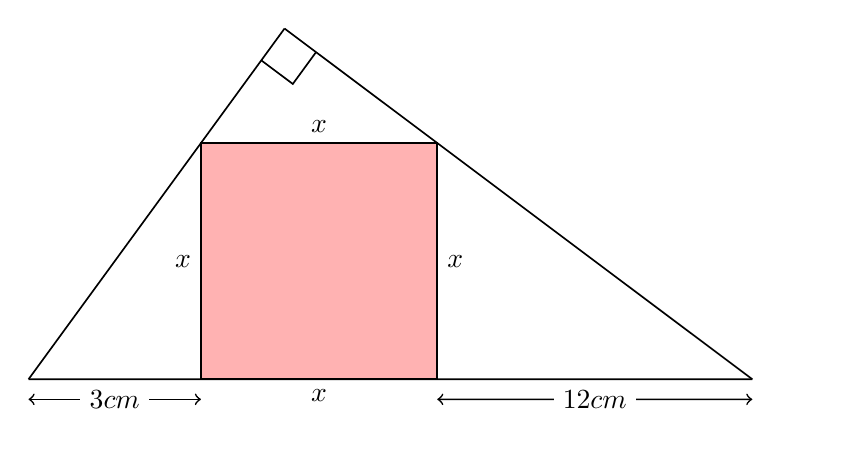
\begin{tikzpicture}[scale=1.5,line width=.6pt]

   

  \draw[fill=red!30,thick] (-1,0) coordinate (a) -- 
        (-1,2) coordinate (b) -- 
        (1,2)  coordinate (c) -- 
        (1,0)  coordinate (d) -- 
        (-1,0);
  
  \node[left]  at ($(a)!.5!(b)$) {$x$};
  \node[above] at ($(c)!.5!(b)$) {$x$};
  \node[right] at ($(c)!.5!(d)$) {$x$};
  \node[below] at ($(a)!.5!(d)$) {$x$};

  \draw (-2.46,0) coordinate (A) -- ($(b)!-1.2cm!(A)$) coordinate (B);
  \path[name path=line1]  (B) -- ($(c)!-4cm!(B)$);
  \path[name path=line2,thick,red] (A) -- (4,0);

  \fill[red, name intersections={of=line1 and line2, by=C}] (C);
  \draw (A) -- (C);
  \draw (B) -- (C);
  
  \pic [draw, angle radius=0.5cm] {right angle = A--B--C};
  \draw[<->] ([yshift=-1.7mm]A) -- ([yshift=-1.7mm]a) node[midway,fill=white] {$3cm$};
  \draw[<->] ([yshift=-1.7mm]d) -- ([yshift=-1.7mm]C) node[midway,fill=white] {$12cm$};


\end{tikzpicture}


\end{document}